\section{Definicija neprekidnosti funkcije}
\begin{definition}[Definicija neprekidnosti funkcije]
Neka je $I\subseteq \mathbb{R}$ otvoreni interval i $c\in I$. Kažemo da je funkcija $f : I\to \mathbb{R}$ \textbf{neprekidna u točki $c$} ako za svaki $\epsilon>0$ postoji $\delta>0$ takav da za sve $x\in I$ vrijedi 
$$|x-c|<\delta\Rightarrow |f(x)-f(c)|<\epsilon.$$
\begin{itemize}
\item $f$ je \textbf{neprekidna na skupu} $S\subseteq I$ ako je ona neprekidna u svakoj točki skupa $S$.
\item $f$ ima \textbf{prekid} u točki $c$ ako ona nije neprekidna u $c$.
\item $f$ ima \textbf{prekid na skupu} $S\subseteq I$ ako postoji bar jedna točka $c\in S$ u kojoj $f$ ima prekid.
\end{itemize}
\end{definition}

\begin{remark}
Gornja definicija može se generalizirati na proizvoljne neprazne skupove $I$.
\end{remark}

\begin{exercise} 
\label{cont1}
Dokažite sljedeće tvrdnje koristeći definiciju neprekidnosti funkcije.
\begin{itemize}
\item[a)] $f : \mathbb{R}\to \mathbb{R}$, $f(x)=3x+4$ je neprekidna u točki $-2$.
\item[b)] $f : \mathbb{R}\to \mathbb{R}$, 
$$f(x)=\begin{cases}
2x, & x\neq 1,\\
1, & x=1,
\end{cases}$$
je neprekidna u svakoj točki $c\neq 1$, a u točki $c=1$ ima prekid.
\end{itemize}
\end{exercise}
\begin{proof}[Rješenje]
a) Treba dokazati da za sve $\epsilon>0$ postoji $\delta>0$ takav da za sve $x\in \mathbb{R}$ vrijedi
$$|x+2|<\delta\Rightarrow |3x+6|=3|x+2|<\epsilon$$
Uzmemo li $\delta=\dfrac{\epsilon}{3}$, tvrdnja vrijedi.

b) Iskoristit ćemo sljedeće slike da bi lakše dokazali tvrdnju.
\begin{figure}[ht]
\begin{subfigure}[t]{.5\textwidth}
\centering
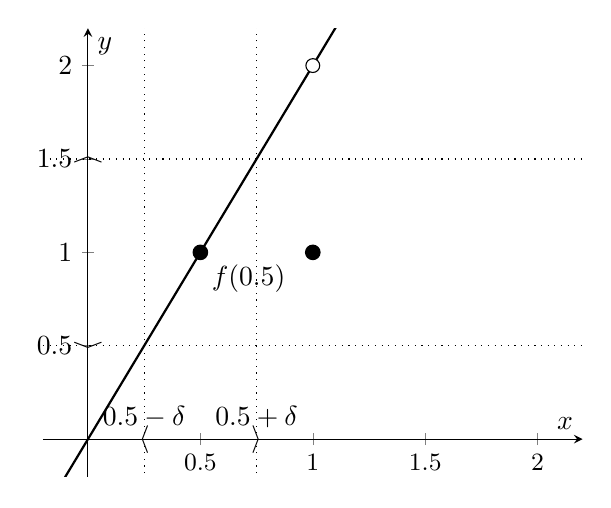
\begin{tikzpicture}
\begin{axis}[axis lines=middle,xlabel=$x$,ylabel=$y$, x tick label style = {font = \small},xmin=-0.2,xmax=2.2,ymin=-0.2,ymax=2.2]

\addplot[thick,color=black,domain=-1.5:3.5] {2*x};
\addplot[dotted,color=black,domain=-1.5:3.5] {0.5};
\addplot[dotted,color=black,domain=-1.5:3.5] {1.5};
\draw[dotted, color=black] (0.25, -1) -- (0.25, 2.5);
\draw[dotted, color=black] (0.75, -1) -- (0.75, 2.5);

\node[circle,draw=black, fill=white, inner sep=0pt,minimum size=5pt] at (1, 2) {};

\node at (axis cs:0.25,0) {$\langle$};
\node at (axis cs:0.75,0) {$\rangle$};
\node[label={[label distance=-0.1cm]-60:$f(0.5)$}] at (axis cs:0.5,1) {};
\node[label={[label distance=-0.1cm]90:$0.5+\delta$}] at (axis cs:0.75,0) {};
\node[label={[label distance=-0.1cm]90:$0.5-\delta$}] at (axis cs:0.25,0) {};
\node[circle,fill,inner sep=2pt] at (axis cs:1, 1) {};
\node[circle,fill,inner sep=2pt] at (axis cs:0.5, 1) {};
\node[rotate=90] at (axis cs:0,0.5) {$\langle$};
\node[rotate=90] at (axis cs:0,1.5) {$\rangle$};
\end{axis}
\end{tikzpicture}
\caption{Neprekidnost funkcije iz zadatka \ref{cont1} u $\frac{1}{2}$}
\end{subfigure}%
\begin{subfigure}[t]{.5\textwidth}
\centering
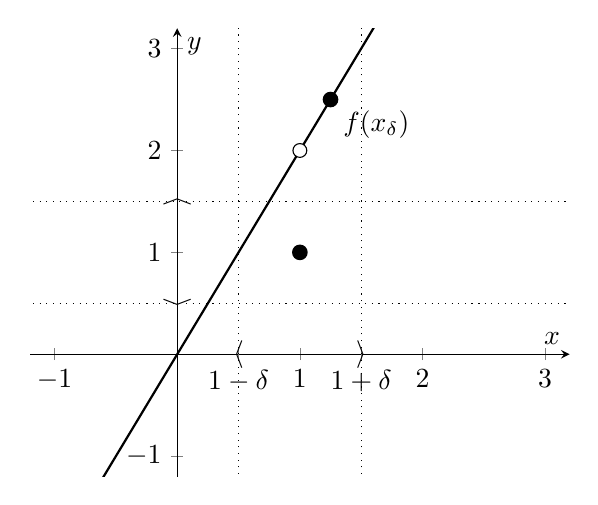
\begin{tikzpicture}
\begin{axis}[axis lines=middle,xlabel=$x$,ylabel=$y$, extra x ticks={0.5, 1.5}, extra x tick labels={$1-\delta$, $1+\delta$},xmin=-1.2,xmax=3.2,ymin=-1.2,ymax=3.2]

\addplot[thick,color=black,domain=-1.5:3.5] {2*x};
\addplot[dotted,color=black,domain=-1.5:3.5] {0.5};
\addplot[dotted,color=black,domain=-1.5:3.5] {1.5};

\node[circle,draw=black, fill=white, inner sep=0pt,minimum size=5pt] at (1, 2) {};

\node at (axis cs:0.5,0) {$\langle$};
\node at (axis cs:1.5,0) {$\rangle$};
\node[label={[label distance=-0.1cm]-30:$f(x_\delta)$}] at (axis cs:1.25,2.5) {};
\node[circle,fill,inner sep=2pt] at (axis cs:1, 1) {};
\node[circle,fill,inner sep=2pt] at (axis cs:1.25, 2.5) {};
\node[rotate=90] at (axis cs:0,0.5) {$\langle$};
\node[rotate=90] at (axis cs:0,1.5) {$\rangle$};
\draw[dotted, color=black] (0.5, -1.5) -- (0.5, 3.5);
\draw[dotted, color=black] (1.5, -1.5) -- (1.5, 3.5);
\end{axis}
\end{tikzpicture}
\caption{Prekid funkcije iz zadatka \ref{cont1} u $1$}
\end{subfigure}
\end{figure}

Primijetimo da za sve $x\in \mathbb{R}$ vrijedi $f(x)=2x$ ako i samo ako je $x\neq 1$, pa moramo odabrati $\delta$ takav da interval $\langle c-\delta, c+\delta\rangle$ ne sadrži broj $1$. Zaista, neka je $\epsilon>0$ proizvoljan. Uzmemo li $$\delta=\min\left \{\dfrac{\epsilon}{2},\; \dfrac{|1-c|}{2}\right\},$$
vrijedi $1\notin \langle c-\delta, c+\delta\rangle$, pa za svaki $x\in \mathbb{R}$ za koji je $|x-c|<\delta$ je $$|2x-2c|=2|x-c|<2\cdot \dfrac{\epsilon}{2}=\epsilon.$$ 
Dokažimo sada da za $c=1$ funkcija ima prekid. Treba dokazati da postoji $\epsilon>0$ takav da za sve $\delta>0$ postoji $x_\delta\in \mathbb{R}$ takav da je 
$$|x_\delta-1|<\delta\;\;\text{ i }\;\;|f(x_\delta)-1|\geq \epsilon.$$ 
Uzmemo li $\epsilon=\dfrac{1}{2}$, $\delta>0$ proizvoljan i $x_\delta=1+\dfrac{\delta}{2}$, imamo 
$$|x_\delta-1|=\dfrac{\delta}{2}<\delta$$ 
i kako je $x_\delta> 1$, slijedi $f(x_\delta)=2x_\delta>2$, pa vrijedi $|f(x_\delta)-1|>1> \epsilon$.
\end{proof}
\begin{remark}
Primijetimo da za sve $x, c\in \mathbb{R}$ i $\delta>0$ takav da je $|x-c|<\delta$ imamo
\begin{gather*}
|c|=|c-x+x|\leq |x-c|+|x|<\delta+|x|,\\
|x|=|x-c+c|\leq |x-c|+|c|,
\end{gather*}
što daje
\begin{gather}
\label{42}
|x|>|c|-\delta,\\
\label{43}
|x|<\delta+|c|.
\end{gather}

\noindent (\ref{42}) daje donju među, a (\ref{43}) gornju među za $|x|$, stoga su ove dvije tvrdnje često korisne kada se treba izraza $|x|$ "riješiti" kako bismo mogli uzeti $\delta$ koji ne ovisi o $x$.
\end{remark}
\begin{exercise}
\label{cont2}
Dokažite sljedeće tvrdnje koristeći definiciju neprekidnosti funkcije.
\begin{itemize}
\item[a)] $f : \mathbb{R}\to \mathbb{R}$, $f(x)=x^2$ je neprekidna na $\mathbb{R}$.
\item[b)] $f : \mathbb{R}\setminus\{0\}\to \mathbb{R}$, $f(x)=\dfrac{1}{x^2}$ je neprekidna na svojoj domeni.
\end{itemize}
\end{exercise}
\begin{proof}[Rješenje]
a) Neka su $c\in \mathbb{R}$ i $\epsilon>0$ proizvoljni. Uzmimo $$\delta=\min\left\{\dfrac{\epsilon}{1+2|c|}, 1\right\}.$$ 
Tada za sve $x\in \mathbb{R}$ takve da je $|x-c|<\delta$ vrijedi 
\begin{gather*}
|x|=|x-c+c|\leq |x-c|+|c|\leq 1+|c|,\\
|x+c|\leq |x|+|c|\leq 1+2|c|.
\end{gather*}
Odavde slijedi
$$|x^2-c^2|=|x-c||x+c|<\dfrac{\epsilon}{1+2|c|}\cdot(1+2|c|)=\epsilon.$$
b) Neka su $c\in \mathbb{R}\setminus\{0\}$ i $\epsilon>0$ proizvoljni. Vrijedi
$$\abs{\dfrac{1}{x^2}-\dfrac{1}{c^2}}=\dfrac{|x^2-c^2|}{|x|^2|c|^2}=\dfrac{|x-c||x+c|}{x^2c^2}$$
Uzmimo
$$\delta=\min\left\{\dfrac{\epsilon\cdot c^4}{4\left(1+2|c|\right)}, 1, \dfrac{|c|}{2}\right\}.$$
Iz (\ref{42}) imamo $$|x|>|c|-\dfrac{|c|}{2}=\dfrac{|c|}{2},\; \text{ tj. }\; x^2>\dfrac{c^2}{4}.$$
Nadalje, kao i u a) dijelu zadatka imamo $|x|+|c|\leq 1+2|c|$. Sve skupa, imamo
$$\dfrac{|x^2-c^2|}{|x|^2|c|^2}=\dfrac{|x-c||x+c|}{x^2c^2}<\dfrac{4|x-c|(1+2|c|)}{c^4}<\epsilon.$$
\end{proof}
\begin{remark}
U b) dijelu zadatka \ref{cont2}, gornju među od $|x+c|$ mogli smo naći i na sljedeći način.

Ako je $c>0$, onda za neki $\delta\leq \dfrac{c}{2}$ imamo
$$|x-c|< \delta\leq \dfrac{c}{2} \Longrightarrow -\dfrac{c}{2}<x-c<\dfrac{c}{2},$$
odakle, zbog činjenice da je $x=|x|$ slijedi
\begin{gather}
\label{44}
\dfrac{c}{2}<|x|<\dfrac{3c}{2},\;\; \dfrac{3c}{2}<|x+c|<\dfrac{5c}{2},
\end{gather}
pa imamo gornju i donju među za $|x+c|$, ali i $|x|$.

Ako je $c<0$, za neki $\delta\leq -\dfrac{c}{2}$  dobivamo $\dfrac{c}{2}<x-c<-\dfrac{c}{2}$, odnosno 
\begin{gather*}
\dfrac{3c}{2}<x<\dfrac{c}{2},\;\; \dfrac{5c}{2}<x+c<\dfrac{3c}{2},
\end{gather*}
no kako je $x\mapsto |x|$ strogo padajuća na $\langle -\infty, 0\rangle$, dobivamo
\begin{gather*}
-\dfrac{c}{2}<|x|<-\dfrac{3c}{2},\;\; -\dfrac{3c}{2}<|x+c|<-\dfrac{5c}{2},
\end{gather*}
dakle opet imamo gornju i donju među za $|x+c|$ i $|x|$.
\end{remark}
\begin{exercise}
Dokažite koristeći definiciju neprekidnosti funkcije da je funkcija $f : \mathbb{R}\to\mathbb{R}$,
$$f(x)=\begin{cases}
-x, & x\in \mathbb{Q},\\
x, & x\in \mathbb{I},
\end{cases}$$
neprekidna u $0$ i ima prekid u svakoj drugoj točki.
\end{exercise}
\newpage
\begin{proof}[Rješenje]
Neka je $\epsilon>0$ proizvoljan. Tada za $\delta=\epsilon$ i za $x\in \mathbb{R}$ takve da je $|x|<\delta$ vrijedi $|f(x)|=|x|<\epsilon,$ čime smo dokazali neprekidnost u $0$.

Dokažimo da $f$ ima prekid u svakoj točki $c>0$. Pretpostavimo sada da je $f$ neprekidna za neki iracionalni $c>0$. Tada tvrdnja vrijedi i za $\epsilon=f(c)$, pa postoji $\delta>0$ takav da za sve $x\in \mathbb{R}$ za koje je $|x-c|<\delta$ vrijedi $|f(x)-f(c)|<f(c)$. Tada vrijedi $$f(x)-f(c)>-f(c),$$ odnosno $f(x)>0$ za sve $x$ za koje je $|x-c|<\delta$. No za $\delta$ zbog gustoće skupa $\mathbb{Q}$ u $\mathbb{R}$, postoji $x_\delta\in \mathbb{Q}$ takav da je $$|x_\delta-c|<\delta.$$ Kako je $x_\delta\in \mathbb{Q}$, vrijedi $f(x_\delta)\leq 0$, što je nemoguće. 

Tvrdnja se analogno dokazuje ako je $x$ racionalan i ako je $c<0$.
\end{proof}
\begin{exercise}
\label{cont4}
Dokažite sljedeće tvrdnje koristeći definiciju neprekidnosti funkcije. 
\begin{itemize}
\item[a)] $f : [0,\infty \rangle\to \mathbb{R}$, $f(x)=\sqrt{x}$ je neprekidna na svojoj domeni.
\item[b)] $f : \mathbb{R} \to \mathbb{R}$, $f(x)=\sin{x}$ je neprekidna na svojoj domeni.
\end{itemize}
\end{exercise}
\begin{proof}[Rješenje]
a) Neka je $\epsilon, c>0$ proizvoljni. Uzmemo li $\delta=\sqrt{c}\epsilon$, za sve $x\geq 0$ za koje je $|x-c|<\delta$ imamo
$$|\sqrt{x}-\sqrt{c}|=\abs{\left(\sqrt{x}-\sqrt{c}\right)\dfrac{\sqrt{x}+\sqrt{c}}{\sqrt{x}+\sqrt{c}}}=\dfrac{|x-c|}{\sqrt{x}+\sqrt{c}}<\dfrac{|x-c|}{\sqrt{c}}<\epsilon$$

b) Neka su $\epsilon>0$ i $c\in \mathbb{R}$ proizvoljni. Uzmemo li $\delta=\epsilon$, za sve $x\in \mathbb{R}$ za koje je $|x-c|<\delta$ vrijedi
$$\abs{\sin{x}-\sin{c}}=\abs{2\cos{\dfrac{x+c}{2}}\sin{\dfrac{x-c}{2}}}\leq 2\abs{\sin{\dfrac{x-c}{2}}},$$
gdje smo iskoristili činjenicu da je $\abs{\cos{\dfrac{x+c}{2}}}\leq 1$. Kako za sve $x\in \mathbb{R}$ vrijedi $\abs{\sin{\dfrac{x-c}{2}}}\leq \abs{\dfrac{x-c}{2}},$ imamo $$2\abs{\sin{\dfrac{x-c}{2}}}\leq |x-c|<\epsilon.$$
\end{proof}
\begin{exercise}
\label{cont3}
Koristeći definiciju neprekidnosti funkcije, odredite najveći\footnote{Najveći skup $S\subseteq \mathbb{R}$ takav da je $f$ neprekidna je skup sa svojstvom da za sve $T\subseteq \mathbb{R}$ za koje je $f$ neprekidna vrijedi $T\subseteq S$.} skup na kojem je funkcija $f : \mathbb{R}\to \mathbb{R}$,
$$f(x)=\begin{cases}
\sqrt{2x-1},& x\geq 1,\\
\dfrac{1}{2}-x,& x<1.
\end{cases}$$
neprekidna.
\end{exercise}
\begin{proof}[Rješenje]

Iz grafa funkcije $f$ vidimo da će ona biti neprekidna svugdje osim u točki $1$. Dokažimo prvo da je $f$ neprekidna na skupu $\mathbb{R}\setminus\{1\}$. 

Zaista, neka je $c>1$ i $$\delta=\min\left\{\dfrac{\sqrt{2c-1}}{2}\epsilon,\; c-1\right\}.$$
Tada za sve $x\in \mathbb{R}$, $|x-c|<c-1$ povlači $x>1$, stoga je 
$$f(x)=\sqrt{2x-1}\;\;\text{ i }\;\;f(c)=\sqrt{2c-1}.$$ 

Neka je $\epsilon>0$ proizvoljan. Slično kao u a) dijelu zadatka \ref{cont4}, za sve $x\in \mathbb{R}$ za koje je $|x-c|<\delta$ vrijedi
\begin{align*}
\abs{\left(\sqrt{2x-1}-\sqrt{2c-1}\right)\cdot\dfrac{\sqrt{2x-1}+\sqrt{2c-1}}{\sqrt{2x-1}+\sqrt{2c-1}}}&=\dfrac{\abs{(2x-1)-(2c-1)}}{\sqrt{2x-1}+\sqrt{2c-1}}\\
&=\dfrac{2|x-c|}{\sqrt{2x-1}+\sqrt{2c-1}}<\dfrac{2|x-c|}{\sqrt{2c-1}}<\epsilon.
\end{align*}

Neka je sada $c<1$ i
$$\delta=\min\left\{\epsilon,\; 1-c\right\}.$$
Dobivamo $|x-c|<1-c$, odakle slijedi $x<1$, pa je $$f(x)=\dfrac{1}{2}-x\;\;\text{ i }\;\;f(c)=\dfrac{1}{2}-c.$$ Neka je $\epsilon>0$ proizvoljan. Za sve $x\in \mathbb{R}$ takve da je $|x-c|<\delta$ vrijedi
$$\abs{\left(\dfrac{1}{2}-x\right)-\left(\dfrac{1}{2}-c\right)}=|x-c|<\epsilon.$$
\newpage
Pokažimo sada da funkcija ima prekid za $c=1$. Uzmimo $\epsilon=\dfrac{1}{2}$ i neka je $\delta>0$ proizvoljan. Uzmimo sada $x_\delta=\max\left\{0,\; 1-\dfrac{\delta}{2}\right\}$. Uočimo da vrijedi 
$$|x_\delta-1|\leq\dfrac{\delta}{2}<\delta.$$
Naime, ako je $1-\dfrac{\delta}{2}\geq 0$, to je jasno, a ako je $1-\dfrac{\delta}{2}\leq 0$, onda je $\delta\geq 2$ i $x_\delta=0$, pa je $$|x_\delta-1|=|0-1|=1\leq\dfrac{\delta}{2}.$$
Kako je $0\leq x_\delta<1$, slijedi $f(x_\delta)=\dfrac{1}{2}-x_\delta\in \left\langle -\dfrac{1}{2}, \dfrac{1}{2}\right]$. To povlači $$|f(x_\delta)-1|\geq \dfrac{1}{2}=\epsilon.$$
\begin{figure}[ht]
\begin{center}
\begin{tikzpicture}
\begin{axis}[axis lines=middle,xlabel=$x$,ylabel=$y$,xmin=-2,xmax=4,ymin=-1,ymax=2.5]

\addplot[thick,color=black,domain=1:4] {sqrt(2*x-1)};
\addplot[thick,color=black,domain=-3:1] {1/2-x};
\node[circle,draw=black, fill=white, inner sep=0pt,minimum size=5pt] at (1, -0.5) {};
\node[circle,fill,inner sep=2pt] at (axis cs:1, 1) {};
\end{axis}
\end{tikzpicture}
\end{center}
\caption{Graf funkcije iz zadatka \ref{cont3}}
\end{figure}
\end{proof}
\section{Svojstva neprekidnih funkcija}
\begin{remark}[Neprekidnost kompozicije funkcija]
\label{compcont}
Neka su $I, I'\subseteq \mathbb{R}$ otvoreni intervali i $f : I\to \mathbb{R}$, $g : I'\to \mathbb{R}$ funkcije takve da je $f(I)\subseteq I'$. Neka je $f$ neprekidna u točki $c\in I$, a $g$ neprekidna u točki $d=f(c)\in I'$. Tada je $h=g\circ f$ neprekidna u točki $c$.
\end{remark}
\begin{remark}[Teorem o lokalnoj ograničenosti neprekidne funkcije]
\label{localbound}
Neka je $I\subseteq \mathbb{R}$ otvoreni interval, $c\in I$ i neka je $f : I\to \mathbb{R}$ neprekidna u $c$. Tada postoje realni brojevi $\eta>0$ i $M>0$ takvi da za sve $x\in I$ vrijedi
$$|x-c|<\eta\Longrightarrow |f(x)|<M.$$
\end{remark}
\begin{remark}[Osnovne operacije s neprekidnim funkcijama]
\label{fundamentalopcont}
Neka je $I\subseteq \mathbb{R}$ otvoreni interval, te neka su $f, g : I\to \mathbb{R}$ neprekidna u točki $c\in I$. Vrijedi:
\begin{itemize}
\item[a)] $f+g$ je neprekidna u $c$,
\item[b)] $fg$ je neprekidna u $c$,
\item[c)] Ako je $g(x)\neq 0$ za sve $x\in I$, onda je $\dfrac{f}{g}$ neprekidna u $c$,
\item[d)] $|f|$ je neprekidna u $c$.
\end{itemize}
\end{remark}
\begin{exercise}
Dokažite napomenu \ref{fundamentalopcont} koristeći definiciju neprekidnosti funkcije.
\end{exercise}
\begin{proof}
a) Budući da su $f$ i $g$ neprekidne u $c$, za svaki $\epsilon>0$ postoje $\delta_1, \delta_2>0$ takvi da za sve $x\in I$ vrijedi
$$|x-c|<\delta_1\Longrightarrow |f(x)-f(c)|<\dfrac{\epsilon}{2}\;\;\text{ i }\;\; |x-c|<\delta_2\Longrightarrow |g(x)-g(c)|<\dfrac{\epsilon}{2}$$
Uzmimo $\delta=\min\{\delta_1, \delta_2\}$. Tada za sve $x\in I$ za koje je $|x-c|<\delta$ vrijedi
\begin{align*}
|(f+g)(x)-(f+g)(c)|&=\abs{\left(f(x)+g(x)\right)-\left(f(c)+g(c)\right)}=\abs{f(x)-f(c)+g(x)-g(c)}\\
&\leq |f(x)-f(c)|+|g(x)-g(c)|<\dfrac{\epsilon}{2}+\dfrac{\epsilon}{2}=\epsilon.
\end{align*}
b) Prema napomeni \ref{localbound} postoje $\eta_1, \eta_2, M_1, M_2>0$ takvi da za sve $x\in I$ vrijedi
$$|x-c|<\eta_1\Longrightarrow |f(x)|<M_1\;\;\text{ i }\;\; |x-c|<\eta_2\Longrightarrow |g(x)|<M_2.$$
Sada za $\eta=\min\left\{\eta_1, \eta_2\right\}$ i $M=\max\left\{M_1, M_2\right\}$ imamo da za sve $x\in I$ takve da je $|x-c|<\eta$ vrijedi $|f(x)|, |g(x)|<M$. Nadalje, zbog neprekidnosti od $f$ i $g$, za svaki $\epsilon>0$ postoje $\delta_1, \delta_2>0$ takvi da za sve $x\in I$ vrijedi
$$|x-c|<\delta_1\Longrightarrow |f(x)-f(c)|<\dfrac{\epsilon}{2M}\;\;\text{ i }\;\; |x-c|<\delta_2\Longrightarrow |g(x)-g(c)|<\dfrac{\epsilon}{2M}.$$
Uzmimo $\delta=\min\{\delta_1, \delta_2, \eta\}$. Tada je
\begin{align*}
|(fg)(x)-(fg)(c)|&=\abs{f(x)g(x)-f(c)g(c)}\\
&=\abs{f(x)g(x)-f(c)g(x)+f(c)g(x)-f(c)g(c)}\\
&\leq |f(x)-f(c)||g(x)|+|g(x)-g(c)||f(c)|<\dfrac{\epsilon}{2M}\cdot M+\dfrac{\epsilon}{2M}\cdot M=\epsilon.
\end{align*}
c) Nije teško pokazati da je funkcije $q : I\setminus\{0\}\to \mathbb{R}$, $q(x)=\dfrac{1}{x}$ neprekidna na svojoj domeni. Uočimo da je $\dfrac{1}{g}=q\circ g$. Za sve $c\in I\setminus\{0\}$ vrijedi $g(c)\neq 0$, pa je, po napomeni \ref{compcont} i $\dfrac{1}{g}=q\circ g$ neprekidna u $c$. No i $f$ je neprekidna u $c$, pa je prema b), $f\cdot \dfrac{1}{g}=\dfrac{f}{g}$ neprekidna u $c$, dakle i neprekidna na $I\setminus\{0\}$.

d) Lako je pokazati da je $q : \mathbb{R}\to \mathbb{R}$, $q(x)=|x|$ neprekidna na $\mathbb{I}$. Kako je $f$ neprekidna na $\mathbb{R}$, slijedi i da je $q\circ f=|f|$ neprekidna na $\mathbb{R}$.
\end{proof}
\begin{remark}[Heineova karakterizacija neprekidnosti]
Neka je $I\subseteq \mathbb{R}$ otvoreni interval i neka je zadana $f : I\to \mathbb{R}$. Funkcija $f$ je neprekidna u točki $c\in I$ ako i samo ako za svaki niz $(a_n)$ iz $I$ koji konvergira prema $c$, niz $\left(f(a_n)\right)$ konvergira prema $f(c)$.
\end{remark}

Prethodna činjenica je vrlo korisna kako bi pokazali da neka funkcija ima prekid u nekoj točki.
\begin{exercise} Dokažite: Funkcija $f : \mathbb{R}\to \mathbb{R}$, $$f(x)=\begin{cases}
2x-1,\; x\leq 3,\\
-x+6,\; x>3.
\end{cases}$$
ima prekid u točki $c=3$.
\end{exercise}
\begin{proof}[Rješenje]
Dovoljno je pokazati da postoji niz $(a_n)$ realnih brojeva koji konvergira u $3$ takav da $\left(f(a_n)\right)$ ne konvergira u $f(3)=5$. Promotrimo niz $(a_n)$ zadan formulom $a_n=3+\dfrac{1}{n}$. Tada je $\lim\limits_{n\to \infty}{a_n}=3$, te kako je $a_n>3$ za sve $n\in \mathbb{N}$, za niz $\left(f(a_n)\right)$, gdje je
$$f(a_n)=-\left(\dfrac{1}{n}+3\right)+6=9-\dfrac{1}{n}$$
vrijedi $\lim\limits_{n\to \infty}{f(a_n)}=9\neq 5$, što je i trebalo pokazati.
\end{proof}
\begin{exercise}
Zadana je funkcija $f : \mathbb{R}\to \mathbb{R}$,
$$f(x)=\begin{cases}
-2, & x<0,\\
1, & x\geq 0.
\end{cases}$$
Dokažite da je ona neprekidna u svakoj točki $c\neq 0$ koristeći Heineovu karakterizaciju neprekidnosti.
\end{exercise}
\begin{proof}
Uzmimo npr. da je $c>0$, slučaj $c<0$ tretira se analogno. Uzmimo proizvoljan niz $(a_n)$ takav da je $\lim\limits_{n\to \infty}{a_n}=c$. Iz definicije slijedi da postoji $n_0\in \mathbb{R}$ takav da za sve prirodne $n\geq n_0$ vrijedi $|a_n-c|<c$, odakle slijedi da je $a_n>0$ za sve $n\geq n_0$. Zato je $f(a_n)=1=f(c)$ za sve $n\in \mathbb{N}$ osim za njih konačno mnogo, pa je jasno da je $\lim\limits_{n\to \infty}{a_n}=1$.
\end{proof}

\begin{exercise}
Zadana je funkcija $f : [0, 1]\to \mathbb{R}$, $$f(x)=\begin{cases}
1, \; x=0,\\
\dfrac{1}{n},\; x=\dfrac{m}{n}\in \mathbb{Q}\setminus\{0\},\mathrm{gdje\;su\;}m\in \mathbb{Z}\mathrm{\;i\;}n\in \mathbb{N}\mathrm{\;relativno\;prosti.}\\
0,\; x\in \mathbb{I}.
\end{cases}$$
Ova funkcija zove se \textit{Thomaeova funkcija}. Dokažite da je ona neprekidna u svakoj iracionalnoj točki i ima prekid u svakoj racionalnoj točki.
\end{exercise}
\begin{proof}[Rješenje]
Dokažimo sljedeću pomoćnu tvrdnju: Neka je $M>0$ proizvoljan. Tada je skup
$$S_M=\left\{x\in[0, 1] : f(x)\geq M\right\}$$
konačan. 

Zaista, ako je $M>1$, vrijedi $S_M=\emptyset$. 

Ako je $M\leq 1$, iz $f(x)\geq M>0$ slijedi da je ili $x=1$ (pa je $S_M$ konačan) ili postoji $n\in \mathbb{N}$ takav da je $f(x)=\dfrac{1}{n}$. Uočimo da je $$\dfrac{1}{n}\geq M\Longleftrightarrow n\leq \dfrac{1}{M},$$ pa je $\left\{n\in \mathbb{N} : \dfrac{1}{n}\geq M\right\}$ odozgo ograničen podskup skupa $\mathbb{N}$, dakle on je konačan. To znači da za sve $x\in S_M$ vrijedi ili $x=0$, ili postoje $m\in \mathbb{Z}$ i $n\in \mathbb{N}$ takvi da je $x=\dfrac{m}{n}$, kojih je očito konačno mnogo, jer je $n\in \left\{1, 2,\dots, \dfrac{1}{M}\right\}$, te $m\in \{1, \dots, n\}$.

Pokažimo sada neprekidnost funkcije u svakoj iracionalnoj točki. Neka su $\epsilon>0$ i $c\in \mathbb{I}$ proizvoljni. Tvrdimo da postoji $\delta>0$ takav da za sve $x\in \mathbb{R}$ vrijedi $$|x-c|<\delta\Rightarrow |f(x)|=f(x)<\epsilon.$$ 
Ako je $\epsilon\geq 1$, tvrdnja je trivijalna. Uzmimo zato $\epsilon<1$. Očito je tada skup $S_\epsilon$ neprazan, jer je npr. $0\in S_\epsilon$.

Neka je $x_0\in S_\epsilon$ točka takva da za sve $y\in S_\epsilon$ vrijedi $|x_0-c|\leq|y-c|$. Takva točka postoji, jer inače bi slično kao u rješenju zadatka \ref{limitpoints3} dobili da je $S_\epsilon$ beskonačan, što očito ne vrijedi. Tvrdimo da za $\delta=|x_0-c|$, ne postoji $x\in \mathbb{R}$ takav da je $|x-c|<\delta$ i $x\in S_\epsilon$. Zaista, u tom slučaju bi imali $$|x_0-c|\leq |x-c|<\delta=|x_0-c|,$$ kontradikcija! Ovo povlači da za sve $x\in \mathbb{R}$ takve da je $|x-c|<\delta$ vrijedi $|f(x)|<\epsilon$, što je i trebalo pokazati.

Dokažimo sada da funkcija ima prekid u svakoj racionalnoj točki. Zaista, ako je $q\in \mathbb{Q}$, onda je $f(q)\neq 0$, a kako za svaki broj $q$ postoji niz $(a_n)$ iracionalnih brojeva koji konvergira prema $q$ (Dokažite to!), za taj niz je $\lim\limits_{x\to \infty}{f(a_n)}=0\neq f(q)$, čime smo dokazali tvrdnju.
\end{proof}
\begin{remark}[Bolzano-Weierstrassov teorem]
Neka je $f : [a, b]\to \mathbb{R}$ neprekidna funkcija na segmentu $[a, b]$. Tada je $f([a, b])$ također segment.
\end{remark}
\begin{remark}
Neka je $f : [a, b]\to \mathbb{R}$ neprekidna funkcija na segmentu $[a, b]$. Prethodni teorem je ekvivalentan s konjunkcijom sljedeće tri tvrdnje.
\begin{itemize}
\item $f$ je ograničena na $[a, b]$, tj. postoji $M\in \mathbb{R}$ takav da je $|f(x)|\leq M$ za sve $x\in [a, b]$.
\item $f$ dostiže svoj infimum i supremum na $[a, b]$, tj. postoje $x_m, x_M\in [a, b]$ za koje je\footnote{Ako je $S\neq \emptyset$ i $f : S\to \mathbb{R}$, onda se $\inf{f}, \sup{f}, \min{f}, \max{f}$ definiraju kao $\inf{\mathcal{R}(f)}, \sup{\mathcal{R}(f)}, \min{\mathcal{R}(f)}, \max{\mathcal{R}(f)}$, respektivno.} 
\begin{gather*}
f(x_m)=\inf{f}=\min{f}=m,\\
f(x_M)=\sup{f}=\max{f}=M.
\end{gather*}
\item (Teorem o međuvrijednostima) Za svaki $C\in [m, M]$ postoji $c\in [a, b]$ takav da je $C=f(c)$.
\end{itemize}
\end{remark}
\newpage
\begin{exercise}
\label{imgcont1}
Zadana je $f : [0, 2]\to \mathbb{R}$, $f(x)=x^5+3x^3$. Odredite $\mathcal{R}(f)$.
\end{exercise}
\begin{proof}[Rješenje]
Uočimo da su $f_1 : [0, 2]\to \mathbb{R}$, $f(x)=x^5$ i $f_2 : [0, 2]\to \mathbb{R}$, $f_2(x)=3x^3$ strogo rastuće, pa je i $f=f_1+f_2$ strogo rastuća. Zato je $$f(0)=0=\min{f}\;\;\text{ i }\;\;f(2)=56=\max{f},$$
pa je $\mathcal{R}(f)\subseteq [0, 56]$.

S druge strane, može se pokazati da je $x\mapsto x^n$ je neprekidna na $\mathbb{R}$ za sve $n\in \mathbb{N}$ (v. \cite{3}), odakle slijedi i da je $f$ neprekidna na $\mathbb{R}$, te je specijalno $f$ neprekidna na $[0, 2]$. Iz teorema o međuvrijednostima imamo da za sve $C\in [0, 56]$ postoji $c\in [0, 2]$ takav da je $C=f(c)$. Odavde slijedi $[0, 56]\subseteq \mathcal{R}(f)$, pa je $\mathcal{R}(f)=[0, 56]$.
\end{proof}
\begin{exercise}
Zadana je $f : \mathbb{R}\to \mathbb{R}$, $f(x)=x\sin{x}$. Odredite $\mathcal{R}(f)$.
\end{exercise}
\begin{proof}[Rješenje]
Neka je $n\in \mathbb{N}$ proizvoljan. Kako je $f$ neprekidna na $\mathbb{R}$, ona je i neprekidna na segmentu $\left[-\dfrac{\pi}{2}-2n\pi, \dfrac{\pi}{2}+2n\pi\right]$. Uočimo da za sve $x\in \left[-\dfrac{\pi}{2}-2n\pi, \dfrac{\pi}{2}+2n\pi\right]$ vrijedi 
$$|x\sin{x}|=|x||\sin{x}|\leq |x|\leq \dfrac{\pi}{2}+2n\pi$$
i vrijedi $f\left(\dfrac{\pi}{2}+2n\pi\right)=\dfrac{\pi}{2}+2n\pi$, pa je $$\min{f}=-\dfrac{\pi}{2}-2n\pi\;\;\text{ i }\;\;\max{f}=\dfrac{\pi}{2}+2n\pi.$$
Odavde, slično kao u zadatku \ref{imgcont1}, slijedi $$f\left(\left[-\dfrac{\pi}{2}-2n\pi, \dfrac{\pi}{2}+2n\pi\right]\right)=\left[-\dfrac{\pi}{2}-2n\pi, \dfrac{\pi}{2}+2n\pi\right].$$
Neka je sada $y\in \mathbb{R}$ proizvoljan. Prema Arhimedovu aksiomu postoje $n_0, m_0\in \mathbb{N}$ takav da je 
$$n_0>\dfrac{y-\dfrac{\pi}{2}}{2}\;\;\text{ i }\;\; m_0>-\dfrac{y+\dfrac{\pi}{2}}{2\pi},$$
odnosno
$$\dfrac{\pi}{2}+2n_0\pi>y\;\;\text{ i }\;\;-\dfrac{\pi}{2}-2m_0\pi<y,$$
odakle za $n_1=\max\{n_0, m_0\}$ slijedi da je $y\in \left[-\dfrac{\pi}{2}-2n_1\pi, \dfrac{\pi}{2}+2n_1\pi\right]$. Međutim, kako je $f$ neprekidna na $\left[-\dfrac{\pi}{2}-2n_1\pi, \dfrac{\pi}{2}+2n_1\pi\right]$, postoji $x\in \mathbb{R}$ takav da je $y=f(x)$. Dakle, vrijedi $\mathbb{R}\subseteq \mathcal{R}(f)$, što znači da je $\mathcal{R}(f)=\mathbb{R}$.
\end{proof}
\begin{exercise}
Neka je $I\subseteq \mathbb{R}$ otvoreni interval i neka je $f : I\to \mathbb{R}$ neprekidna i strogo monotona na $I$. Dokažite da je tada $\mathcal{R}(f)$ otvoreni interval.
\end{exercise}
\begin{proof}
Uzmimo da $f$ strogo raste na $I$ (Analogno se tretira slučaj gdje $f$ strogo pada). Pretpostavimo da je $\inf{\mathcal{R}(f)}=\inf{f}\in \mathcal{R}(f)$. Tada postoji $a\in I$ takav da je $f(a)=\inf{f}$. Međutim, kako je $I$ otvoreni interval, postoji $a'\in I$ takav da je $a'<a$. Odavde je $f(a_1)\in \mathcal{R}(f)$ i vrijedi $f(a_1)<f(a)=\inf{f}$, kontradikcija! Analogno se pokazuje da $\sup{f}\notin \mathcal{R}(f)$. Odavde dobivamo $\mathcal{R}(f)\subseteq \langle \inf{f}, \sup{f} \rangle$.

Neka je $z\in \langle \inf{f}, \sup{f} \rangle$. Tada postoje $x, y\in \langle \inf{f}, \sup{f} \rangle$ takvi da je $x<z<y$. Kako je $f$ strogo rastuća, ona ima inverznu funkciju $f^{-1}$ koja je također strogo rastuća, pa je $f^{-1}(x)<f^{-1}(z)<f^{-1}(y)$. No tada je $f\left(\left[f^{-1}(x), f^{-1}(y)\right]\right)$ segment, pa je $$z\in f\left(\left[f^{-1}(x), f^{-1}(y)\right]\right)\;\;\text{ i }\;\;f\left(\left[f^{-1}(x), f^{-1}(y)\right]\right)\subseteq f(I)=\mathcal{R}(f),$$
što vrijedi zbog činjenice da za svaku funkciju $g : S\to \mathbb{R}$ i skupove $A\subseteq B\subseteq S$ vrijedi $f(A)\subseteq f(B)$ (Dokažite to!).
Dobivamo $z\in \mathcal{R}(f)$, pa zaključujemo da je $\mathcal{R}(f)=\langle \inf{f}, \sup{f}\rangle$.
\textbf{NADOPUNITI SLUCAJ KAD SLIKA NIJE OGRANICEN SKUP}
\end{proof}
\newpage
\section*{Zadatci za vježbu}
\begin{exercise}
Koristeći definiciju neprekidnosti funkcije, dokažite sljedeće tvrdnje: 
\begin{itemize}
\item[a)] $x\mapsto |3x+2|$ je neprekidna na $\mathbb{R}$,
\item[b)] $x\mapsto x(x+1)$ je neprekidna na $\mathbb{R}$,
\item[c)] $x\mapsto x^3$ je neprekidna na $\mathbb{R}$,
\item[d)] $x\mapsto \dfrac{1}{\sqrt{x}}$ je neprekidna na $\mathbb{R}^+$,
\item[e)] $x\mapsto \sqrt{x^2+1}$ je neprekidna u $0$,
\item[f)] $f : \mathbb{R}\to \mathbb{R}$, $$f(x)=\begin{cases}
x\sin{\dfrac{1}{x}}, & x\neq 0,\\
0, & x=0,
\end{cases}
$$ 
je neprekidna u $0$,
\item[g)] $x\mapsto 2\sin^2{x}-1$ je neprekidna na $\mathbb{R}$.
\end{itemize}
\end{exercise}
\begin{exercise}
Zadan je otvoreni interval $I\subseteq \mathbb{R}$ i funkcija $f : I\to \mathbb{R}$. Dokažite ili opovrgnite: $f$ je neprekidna u $c$ ako i samo ako...
\begin{itemize}
\item[a)] Postoji $\delta>0$ takav da za sve $\epsilon>0$ i sve $x\in I$ vrijedi $|x-c|<\delta\Rightarrow |f(x)-f(c)|<\epsilon$,
\item[b)] Za svaki $\epsilon>0$ postoji $\delta>0$ takav da za sve $x\in I$ vrijedi $|f(x)-f(c)|<\epsilon\Rightarrow |x-c|<\delta$,
\item[c)] Za svaki $\delta>0$ postoji $\epsilon>0$ takav da za sve $x\in I$ vrijedi $|x-c|<\delta\Rightarrow |f(x)-f(c)|<\epsilon$.
\end{itemize}
\end{exercise}
\begin{exercise}
Neka je $I\subseteq \mathbb{R}$ otvoreni interval i $c\in I$. Zadana je funkcija $f : I\to \mathbb{R}$ sa sljedećim svojstvom: Za svaki $k\in \mathbb{N}$ postoji $\delta>0$ tako da za sve $x\in I$ vrijedi $|x-c|<\delta\Rightarrow |f(x)-f(c)|<\dfrac{1}{2^k}$. Dokažite ili opovrgnite: $f$ je neprekidna u $c$.
\end{exercise}
\begin{exercise}
Postoji li $c\in \mathbb{R}$ takav da vrijedi:
\begin{itemize}
\item[a)] $f : \mathbb{R}\to \mathbb{R}$, $$f(x)=\begin{cases}
\arctg{\dfrac{1}{x-1}},& x\neq 1,\\
c, & x=1
\end{cases}$$ 
je neprekidna u $1$.
\item[b)] Funkcija $f : \mathbb{R}\to \mathbb{R}$, $$f(x)=\begin{cases}
2x-c,& x\leq 1,\\
\sqrt{x-1},& x>1.
\end{cases}$$
je neprekidna u $1$.
\item[b)] $f : \mathbb{R}\to \mathbb{R}$, $$f(x)=\begin{cases}
\sin{\dfrac{1}{x}},\; x\neq 0,\\
c,\; x=0.
\end{cases}$$
je neprekidna u $0$.
\end{itemize}
\end{exercise}
\begin{exercise}
Koristeći definiciju neprekidnosti funkcije, odredite najveći skup na kojem je funkcija $f : \mathbb{R}\to \mathbb{R}$,
$$f(x)=\begin{cases}
x^2,& x\leq 3,\\
2x+1,& x>3.
\end{cases}$$
neprekidna.
\end{exercise}
\begin{exercise}
Dokažite da je $\mathcal{R}(\sin)=\mathcal{R}(\cos)=[-1, 1]$ i da je $\mathcal{R}(\tg)=\mathbb{R}$.
\end{exercise}
\begin{center}
$*\hspace{0.3cm}*\hspace{0.3cm}*\hspace{0.3cm}$
\end{center}
\begin{exercise} $(*)$
Koristeći definiciju neprekidnosti funkcije, dokažite da je $\sqrt[3]{x}$ neprekidna na svojoj domeni.
\end{exercise}
\begin{exercise} $(**)$
Dokažite da polinom $f : \mathbb{R}\to \mathbb{R}$, $f(x)=a_nx^n+\dots+a_1x+a_0$ neparnog stupnja ima bar jednu nultočku.
\end{exercise}